\subsection{Architektury OS}

\begin{obecne}{Klasická struktura~-- monolitická}
Nejstarší, už IBM 360, Unix, Win., všechny služby uvnitř, prováděny ve chráněném módu, jádro poměrně velké, \uv{údajně} nejrychlejší. Program zavolá službu OS, přes tabulku se zjistí adresa přísl. fce, ta se zavolá a vrátí výsledek.  Nevýhoda: horší údržba -- je-li v programu chyba, může poškodit zbývající části systému, rozšiřování za běhu je komplikované. 
\end{obecne}

\begin{obecne}{Virtuální stroje}
Původní nápad : Virtual Machine pro IBM360 -- oddělit multitasking od OS jako ext. stroj. Nad HW byla další vrstva -- \uv{Virtual Machine} -- měla plánovat, vyrábí pro procesy iluzi holého HW; dneska např. VMWare dělá to samé. Pro IBM360 se dalo použít v kombinaci s CMS (jednoúlohový) i původního OS360 (rychlejší než OS360 na holém HW). 

Dnes: definuji abstraktní stroj, pro něj překládám programy (.NET, Java) $\rightarrow$ přenositelnost, kompatibilita (IBM AS400~-- desítky let), problém~-- pomalé. 
\end{obecne}

\begin{obecne}{Mikrojádro}
snaha aby část běžící v kernel módu byla co nejmenší (třeba jen cca 10 KB), nejnovější, experimentální, často pro Distribuované OS (dnes už nepoužívané), hodně procesů \& komunikace (klient/server), mikrojádro řeší jenom komunikaci. 

Filesystém apod. jsou procesy -- aplikace jim posílají přes jádro požadavky. Jediný komerční OS -- Chorus (ústředny). výhoda: když něco spadne, nepoškodí to zbytek, moduly jdou měnit za běhu, komunikace jde snadno rozšířit na komunikaci po síti. 
\end{obecne}

\begin{obecne}{Architektura WinNT}
  Jádro je poměrně malé (cca 1MB), schopné (pro vyšší vrstvy jsou některé schopnosti skryté), na jeho vzniku se podíleli schopní Unixáři. Byla zde snaha o malou velikost, přenositelnost. Jádro je neutrální vzhledem k vyšším vrstvám, nad ním lze vybudovat různé systémy (Windows subsystém, POSIX, OS/2).

  Rozhraní OS a uživ. programů zajišťuje WinAPI, nad ním se nacházejí různé DLL, mezi kernelem a HW je \uv{hardware abstraction layer}, tj. kernel lze jednoduše upravit pro jiné architektury (Alpha, IA-64).
  Grafické drivery jediné mají přímý přístup k HW (kvůli výkonu), části API (USER, GDI) jsou implementované v jádře, přechod mezi user a kernel režimem zajišťuje ntdll.dll (a je tedy využíván všemi programy). Veškeré služby a aplikace běží v user módu nad jádrem.

  \begin{center}
    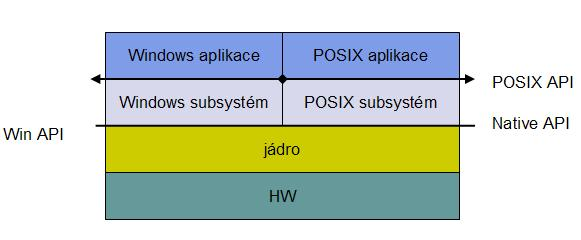
\includegraphics[width=8cm]{informatika/operacne_systemy_a_hw/obrazky/arch-windows.jpg}
  \end{center}
\end{obecne}

\begin{obecne}{Architektura Linuxu}
  \begin{pitemize}
      \item Na úrovni SW -- přenositelnost; abstrakce HW. 
      \item nad HW~-- kernel, nad ním systémová volání, hodně podobné Windows.
  \end{pitemize}

  \begin{center}
    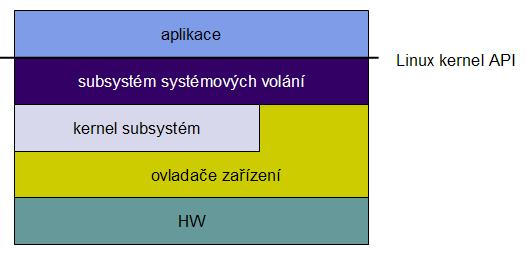
\includegraphics[width=8cm]{informatika/operacne_systemy_a_hw/obrazky/arch-linux.jpg}
  \end{center}
\end{obecne}
